\documentclass[aspectratio=169, table]{beamer}

\usepackage{array}
\usepackage{colortbl}
\usepackage{tabularx}
\usepackage{xcolor}
\usepackage{tikz}
\usetikzlibrary{arrows.meta, positioning, calc, fit}

\makeatletter
\def\input@path{{../theme/}}
\makeatother
\graphicspath{{../theme/}}
\usetheme{Pradita}

\newcommand{\sectionframe}[1]{%
  \begin{frame}{\hfill}
    \centering
    \Huge{\textbf{#1}}
  \end{frame}
}

\newcommand{\takeaway}[1]{%
  \vspace{4pt}
  {\footnotesize #1}
}

\title{\huge Orientasi EA dan Platform\\
  \vspace{8pt}
  + Penulisan Akademik}
\subtitle{IT30713 - Enterprise \& Platform Architecture}
\author{\textbf{Alfa Yohannis}}
\date{30 Mei 2026}

\begin{document}

\frame{\titlepage}

\begin{frame}[fragile]
  \frametitle{Contents}
  \vspace{20pt}
  \begin{columns}[t]
    \column{0.5\textwidth}
    \tableofcontents[sections={1-4}]

    \column{0.5\textwidth}
    \tableofcontents[sections={5-8}]
  \end{columns}
\end{frame}

\begin{frame}{\hfill}
  \centering
  \Huge{\textbf{Bagaimana strategi organisasi\\menjadi keputusan arsitektur?}}
\end{frame}

\section{Orientasi Bab}
\sectionframe{Orientasi Bab}

\begin{frame}{Tujuan Pembelajaran}
  \vspace{8pt}
  \begin{itemize}
    \item Menjelaskan \textbf{Enterprise Architecture} sebagai jembatan antara strategi organisasi dan kapabilitas teknologi.
    \item Membedakan domain \textbf{Business, Data, Application, Technology} serta peran API dan platform.
    \item Mengenali anatomi makalah ilmiah untuk topik Enterprise Architecture, API, dan platform.
    \item Menyusun topik awal, memilih organisasi studi kasus Indonesia, dan mengidentifikasi kandidat publikasi.
  \end{itemize}

  \takeaway{Arah sesi: memahami peta besar mata kuliah sekaligus memulai bahan makalah individual}
\end{frame}

\begin{frame}{Tiga Gagasan Utama}
  \vspace{10pt}
  \begin{columns}[t]
    \column{0.32\textwidth}
    \textbf{EA sebagai cara berpikir}
    \vspace{4pt}
    \begin{itemize}
      \item Membaca organisasi sebagai sistem.
      \item Menghubungkan tujuan, proses, data, aplikasi, dan teknologi.
    \end{itemize}

    \column{0.32\textwidth}
    \textbf{Platform dan API}
    \vspace{4pt}
    \begin{itemize}
      \item Membuka integrasi dan kolaborasi.
      \item Mengubah posisi organisasi dalam ekosistem digital.
    \end{itemize}

    \column{0.32\textwidth}
    \textbf{Makalah publikasi}
    \vspace{4pt}
    \begin{itemize}
      \item Mengubah analisis menjadi kontribusi akademik.
      \item Dibangun bertahap selama satu semester.
    \end{itemize}
  \end{columns}

  \takeaway{Bab 1 menyatukan konsep arsitektur, konteks bisnis digital, dan target tulisan ilmiah}
\end{frame}

\begin{frame}{Skenario Pembuka}
  \vspace{14pt}
  \begin{columns}[T,onlytextwidth]
    \begin{column}{0.47\textwidth}
    \small
    \begin{itemize}
      \item Bank daerah dengan jaringan cabang tradisional ingin memperkuat layanan digital.
      \item Agenda transformasi mencakup aplikasi mobile, QRIS, kemitraan fintech, dan API publik untuk UMKM.
      \item Direksi sepakat pada tujuan, tetapi belum sepakat pada urutan, prioritas, dan risiko.
    \end{itemize}
    \end{column}

    \begin{column}{0.50\textwidth}
    \centering
    \resizebox{\linewidth}{!}{
      \begin{tikzpicture}[
        font=\small\bfseries,
        actor/.style={draw, rounded corners=1.5mm, align=center, minimum width=30mm, minimum height=8mm, fill=blue!10},
        bank/.style={actor, fill=praditagreen!22, minimum width=34mm, minimum height=11mm},
        arrow/.style={-Latex, thick}
      ]
        \node[bank] (bank) {Bank\\Wanua};
        \node[actor, above left=of bank] (nasabah) {Nasabah\\lokal};
        \node[actor, above right=of bank] (umkm) {UMKM};
        \node[actor, below left=of bank] (fintech) {Fintech};
        \node[actor, below right=of bank] (reg) {BI, OJK,\\UU PDP};

        \draw[arrow] (bank) -- (nasabah);
        \draw[arrow] (bank) -- (umkm);
        \draw[arrow] (bank) -- (fintech);
        \draw[arrow] (reg) -- (bank);
      \end{tikzpicture}
    }
    \end{column}
  \end{columns}

  \vfill
  \takeaway{Pertanyaan transformasi digital jarang dapat dijawab hanya sebagai keputusan teknis}
\end{frame}

\begin{frame}{Pertanyaan Pemandu}
  \vspace{10pt}
  \begin{enumerate}
    \item Apa makna Enterprise Architecture, dan mengapa penting bagi audiens non-IT?
    \item Bagaimana platform dan API mengubah keputusan arsitektur organisasi?
    \item Apa yang membedakan makalah ilmiah dari laporan proyek atau dokumen konsultasi?
    \item Bagaimana memilih target publikasi yang realistis dan relevan?
    \item Bagaimana memulai semester dengan studi kasus dan topik makalah yang tepat?
  \end{enumerate}

  \takeaway{Kelima pertanyaan ini menjadi kompas dari konsep menuju tugas individual}
\end{frame}

\begin{frame}{Mengapa Penting bagi Non-IT}
  \vspace{10pt}
  \begin{itemize}
    \item Keputusan arsitektur enterprise menyentuh bisnis, anggaran, regulasi, SDM, budaya, dan risiko.
    \item Strategi digital sering gagal ketika keputusan teknis tidak tersambung dengan keputusan bisnis.
    \item Pengambil keputusan perlu memahami arah, prioritas, tata kelola, dan kompromi arsitektural.
    \item Peran seperti CIO, CDO, Strategy Manager, Product Manager, Business Analyst, dan pemimpin transformasi digital membutuhkan bahasa lintas fungsi.
  \end{itemize}

  \takeaway{EA membantu pemimpin non-IT berdialog dengan tim bisnis, tim TI, dan mitra eksternal}
\end{frame}

\section{EA dan BDAT}
\sectionframe{EA dan BDAT}

\begin{frame}{Empat Pilar Bab Ini}
  \vspace{12pt}
  \centering
  \resizebox{0.9\textwidth}{!}{
    \begin{tikzpicture}[
      font=\small\bfseries,
      block/.style={draw, rounded corners=2mm, align=center, minimum width=31mm, minimum height=18mm},
      arrow/.style={-Latex, very thick}
    ]
      \node[block, fill=praditagreen!22] (ea) {Enterprise\\Architecture};
      \node[block, fill=orange!20, right=6mm of ea] (bdat) {BDAT\\Domains};
      \node[block, fill=blue!12, right=6mm of bdat] (api) {API dan\\Platform};
      \node[block, fill=gray!16, right=6mm of api] (paper) {Makalah\\Ilmiah};

      \draw[arrow] (ea) -- (bdat);
      \draw[arrow] (bdat) -- (api);
      \draw[arrow] (api) -- (paper);
    \end{tikzpicture}
  }

  \vspace{14pt}
  \begin{itemize}
    \item EA memberi cara berpikir.
    \item BDAT memberi lensa analisis.
    \item API dan platform memberi konteks nilai digital.
    \item Makalah ilmiah memberi bentuk komunikasi akademik.
  \end{itemize}
\end{frame}

\begin{frame}{EA sebagai Jembatan}
  \vspace{2pt}
  \centering
  \scalebox{0.84}{
    \begin{tikzpicture}[
      font=\small\bfseries,
      node distance=10mm,
      layer/.style={
        draw, rounded corners=2mm, align=center,
        minimum width=92mm, minimum height=13mm
      },
      strategi/.style={layer, fill=praditagreen!20},
      ea/.style={layer, fill=orange!24, minimum height=17mm},
      tek/.style={layer, fill=blue!12},
      arrow/.style={Latex-Latex, very thick}
    ]
      \node[strategi] (s) {STRATEGI ORGANISASI\\
        \footnotesize\mdseries Visi, model bisnis, tujuan, pelanggan, mitra, regulasi};
      \node[ea, below=of s] (e) {ENTERPRISE ARCHITECTURE\\
        \footnotesize\mdseries Prinsip, kapabilitas, baseline, target, gap, peta jalan};
      \node[tek, below=of e] (t) {KAPABILITAS TEKNOLOGI\\
        \footnotesize\mdseries Aplikasi, data, infrastruktur, integrasi, API, platform};

      \draw[arrow] (s.south) -- (e.north);
      \draw[arrow] (e.south) -- (t.north);

      \node[right=0.4cm of e, align=left, font=\footnotesize\mdseries\itshape, text width=30mm]
        {menerjemahkan\\strategi $\leftrightarrow$\\kapabilitas};
    \end{tikzpicture}
  }

  \takeaway{EA bukan sekadar diagram; EA mendokumentasikan keputusan yang dapat dijelaskan}
\end{frame}

\begin{frame}{Analogi Cetak Biru}
  \vspace{8pt}
  \begin{columns}[t]
    \column{0.48\textwidth}
    \textbf{Cetak biru bangunan}
    \vspace{4pt}
    \begin{itemize}
      \item Membantu pemilik, kontraktor, pekerja, dan pemeriksa berbicara tentang rancangan yang sama.
      \item Memuat pilihan, asumsi, prinsip, urutan kerja, dan biaya.
      \item Tidak menggantikan bangunan, tetapi mengarahkan pembangunannya.
    \end{itemize}

    \column{0.48\textwidth}
    \textbf{Enterprise Architecture}
    \vspace{4pt}
    \begin{itemize}
      \item Membantu direksi, bisnis, TI, regulator, dan mitra menyepakati arah.
      \item Memuat kapabilitas, baseline, target, prinsip, gap, dan roadmap.
      \item Tidak menggantikan implementasi, tetapi membuat keputusan terlihat.
    \end{itemize}
  \end{columns}

  \takeaway{Blueprint adalah bahasa bersama untuk membahas transformasi yang kompleks}
\end{frame}

\begin{frame}{BDAT: Empat Domain Arsitektur}
  \vspace{0pt}
  \centering
  \scalebox{0.82}{
    \begin{tikzpicture}[
      font=\small\bfseries,
      node distance=2mm,
      layer/.style={
        draw, rounded corners=1.5mm, align=left,
        minimum width=112mm, minimum height=11mm,
        inner xsep=4mm
      },
      business/.style={layer, fill=praditagreen!25},
      data/.style={layer, fill=orange!20},
      app/.style={layer, fill=blue!15},
      tech/.style={layer, fill=gray!18}
    ]
      \node[business] (b) {\textbf{B -- BUSINESS}\\
        \footnotesize\mdseries Kapabilitas, value stream, proses, pemangku kepentingan, model operasional};
      \node[data, below=of b] (d) {\textbf{D -- DATA}\\
        \footnotesize\mdseries Entitas data inti, kepemilikan, kualitas, privasi, tata kelola};
      \node[app, below=of d] (a) {\textbf{A -- APPLICATION}\\
        \footnotesize\mdseries Portofolio aplikasi, integrasi, pola layanan, bangun sendiri vs. beli};
      \node[tech, below=of a] (t) {\textbf{T -- TECHNOLOGY}\\
        \footnotesize\mdseries Cloud, infrastruktur, keamanan, prinsip teknologi};
    \end{tikzpicture}
  }

  \takeaway{BDAT memecah kerumitan organisasi tanpa memutus hubungan antar keputusan}
\end{frame}

\begin{frame}{Pertanyaan Kunci per Domain}
  \vspace{10pt}
  \renewcommand{\arraystretch}{1.25}
  \footnotesize
  \begin{tabularx}{\textwidth}{>{\bfseries}p{0.18\textwidth}X}
    \rowcolor{praditagreen!18}
    Domain & Pertanyaan keputusan \\
    Business & Apa yang dilakukan organisasi untuk pelanggan, dan kapabilitas apa yang dibutuhkan? \\
    Data & Informasi apa yang dibutuhkan, siapa pemiliknya, dan bagaimana data dilindungi? \\
    Application & Aplikasi dan layanan apa yang mendukung kapabilitas, dan bagaimana saling terhubung? \\
    Technology & Infrastruktur, keamanan, standar, dan platform teknis apa yang menopang semuanya? \\
  \end{tabularx}

  \vspace{12pt}
  \begin{itemize}
    \item Hampir setiap keputusan transformasi menyentuh keempat domain.
    \item Tugas EA adalah membuat hubungan tersebut terlihat dan dapat dipertanggungjawabkan.
  \end{itemize}
\end{frame}

\section{API dan Platform}
\sectionframe{API dan Platform}

\begin{frame}{Platform Mengubah Alur Nilai}
  \vspace{8pt}
  \begin{columns}[T,onlytextwidth]
    \column{0.42\textwidth}
    \centering
    \textbf{Model linear}
    \par\vspace{2pt}
    \begin{minipage}[t][36mm][c]{\linewidth}
      \centering
      \resizebox{0.95\linewidth}{!}{
        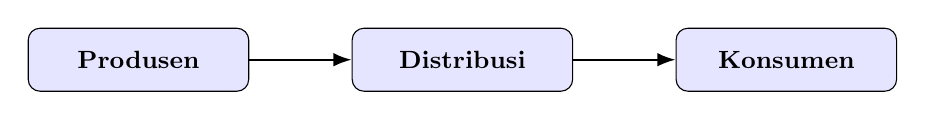
\begin{tikzpicture}[
          font=\small\bfseries,
          box/.style={draw, rounded corners=1.5mm, minimum width=28mm, minimum height=8mm, align=center, fill=blue!10},
          arrow/.style={-Latex, thick}
        ]
          \node[box] (prod) {Produsen};
          \node[box, right=13mm of prod] (dist) {Distribusi};
          \node[box, right=13mm of dist] (kon) {Konsumen};
          \draw[arrow] (prod) -- (dist);
          \draw[arrow] (dist) -- (kon);
        \end{tikzpicture}
      }
    \end{minipage}

    \column{0.52\textwidth}
    \centering
    \textbf{Model platform}
    \par\vspace{2pt}
    \begin{minipage}[t][36mm][c]{\linewidth}
      \centering
      \resizebox{0.95\linewidth}{!}{
        \begin{tikzpicture}[
          font=\small\bfseries,
          box/.style={draw, rounded corners=1.5mm, minimum width=25mm, minimum height=8mm, align=center, fill=blue!10},
          platform/.style={box, fill=praditagreen!22, minimum width=30mm, minimum height=11mm},
          arrow/.style={Latex-Latex, thick}
        ]
          \node[platform] (p) {Platform};
          \node[box, above left=of p] (a) {Pengguna A};
          \node[box, above right=of p] (b) {Pengguna B};
          \node[box, below left=of p] (c) {Mitra};
          \node[box, below right=of p] (d) {Pengembang};
          \draw[arrow] (p) -- (a);
          \draw[arrow] (p) -- (b);
          \draw[arrow] (p) -- (c);
          \draw[arrow] (p) -- (d);
        \end{tikzpicture}
      }
    \end{minipage}
  \end{columns}

  \vspace{10pt}
  \begin{itemize}
    \item Gojek, Tokopedia, BCA Open API, dan BRIAPI menunjukkan nilai yang muncul dari banyak pihak yang saling terhubung.
    \item \textbf{Network effect}: semakin banyak peserta di satu sisi, semakin besar nilai bagi sisi lain.
  \end{itemize}
\end{frame}

\begin{frame}{API sebagai Kontrak Digital}
  \vspace{10pt}
  \begin{itemize}
    \item API membuat satu sistem dapat berinteraksi dengan sistem lain secara terstandar.
    \item Bagi audiens non-IT, API dapat dianalogikan sebagai \textbf{stop kontak}: bentuk dan aturan disepakati agar banyak perangkat dapat terhubung.
    \item API yang baik membuat integrasi mitra lebih cepat, konsisten, aman, dan mudah dikelola.
    \item Dalam platform, API bukan sekadar antarmuka teknis; API adalah alat untuk membangun ekosistem.
  \end{itemize}

  \vspace{8pt}
  \centering
  \scalebox{0.82}{
    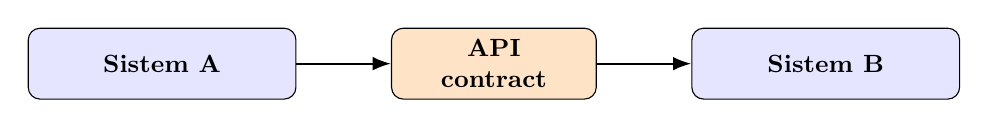
\begin{tikzpicture}[
      font=\small\bfseries,
      box/.style={draw, rounded corners=1.5mm, align=center, minimum width=34mm, minimum height=9mm, fill=blue!10},
      api/.style={box, fill=orange!22, minimum width=26mm},
      arrow/.style={-Latex, thick}
    ]
      \node[box] (sysa) {Sistem A};
      \node[api, right=12mm of sysa] (api) {API\\contract};
      \node[box, right=12mm of api] (sysb) {Sistem B};
      \draw[arrow] (sysa) -- (api);
      \draw[arrow] (api) -- (sysb);
    \end{tikzpicture}
  }
\end{frame}

\begin{frame}{Pilihan Strategis Bank Wanua}
  \vspace{10pt}
  \begin{enumerate}
    \item Menjadi platform mandiri yang mengundang UMKM dan fintech masuk ke ekosistem sendiri.
    \item Bergabung sebagai mitra ke platform yang lebih besar melalui SNAP BI dan dompet digital nasional.
    \item Membuka public API bertahap untuk layanan bernilai tinggi, dengan kontrol keamanan dan kepatuhan yang jelas.
    \item Memperkuat kapabilitas internal sebelum meluncurkan layanan API publik.
  \end{enumerate}

  \takeaway{Keputusan API dan platform menyangkut model bisnis, tata kelola, risiko, dan posisi ekosistem}
\end{frame}

\section{Makalah Ilmiah}
\sectionframe{Makalah Ilmiah}

\begin{frame}{Luaran Utama Mata Kuliah}
  \vspace{10pt}
  \begin{itemize}
    \item Luaran utama adalah \textbf{makalah publikasi individu}.
    \item Digital blueprint enterprise menjadi artefak pendukung, bukan luaran berdiri sendiri.
    \item Artefak seperti capability map, BDAT architecture, API portfolio, platform ecosystem map, governance charter, dan roadmap digunakan sebagai bukti analisis.
    \item Naskah dibangun bertahap dari Sesi 1 sampai Sesi 14.
  \end{itemize}

  \takeaway{Blueprint memperkuat argumen; makalah menyampaikan kontribusi}
\end{frame}

\begin{frame}{Anatomi Makalah}
  \vspace{12pt}
  \centering
  \scalebox{0.64}{
    \begin{tikzpicture}[
      font=\footnotesize\bfseries,
      node distance=1.4mm,
      sec/.style={
        draw, rounded corners=1.2mm, align=left,
        minimum width=112mm, minimum height=5.8mm,
        fill=praditagreen!10,
        inner xsep=3mm
      },
      highlight/.style={sec, fill=orange!22}
    ]
      \node[sec] (a) {Judul, Abstrak, Kata Kunci};
      \node[sec, below=of a] (b) {Pendahuluan: latar belakang, masalah, RQ, kontribusi};
      \node[sec, below=of b] (c) {Tinjauan Pustaka dan Kerangka Konseptual};
      \node[sec, below=of c] (d) {Metode atau Pendekatan Analisis};
      \node[sec, below=of d] (e) {Konteks Organisasi atau Studi Kasus};
      \node[highlight, below=of e] (f) {Analisis Kondisi Saat Ini};
      \node[highlight, below=of f] (g) {Rancangan Arsitektur Target berbasis BDAT};
      \node[highlight, below=of g] (h) {Strategi API dan Strategi Platform};
      \node[highlight, below=of h] (i) {Tata Kelola Platform, Risiko, Metrik};
      \node[highlight, below=of i] (j) {Gap Analysis, Roadmap, Implikasi Manajerial};
      \node[sec, below=of j] (k) {Diskusi, Keterbatasan, Arah Lanjutan};
      \node[sec, below=of k] (l) {Kesimpulan, Rekomendasi, Daftar Pustaka};
    \end{tikzpicture}
  }

  \takeaway{Bagian berwarna oranye menjadi inti kontribusi substantif dari analisis arsitektur}
\end{frame}

\begin{frame}{Fungsi Komunikasi Tiap Bagian}
  \vspace{8pt}
  \begin{columns}[t]
    \column{0.48\textwidth}
    \begin{itemize}
      \item \textbf{Pendahuluan}: meyakinkan pembaca bahwa masalah penting.
      \item \textbf{Tinjauan pustaka}: menempatkan makalah dalam percakapan akademik.
      \item \textbf{Metode}: menjelaskan cara analisis agar dapat dievaluasi.
    \end{itemize}

    \column{0.48\textwidth}
    \begin{itemize}
      \item \textbf{Analisis dan rancangan}: menyajikan kontribusi inti.
      \item \textbf{Diskusi}: mengubah temuan menjadi makna dan implikasi.
      \item \textbf{Kesimpulan}: menutup argumen dan menunjukkan arah lanjutan.
    \end{itemize}
  \end{columns}

  \takeaway{Makalah ilmiah berbeda dari laporan proyek karena argumennya harus dapat ditelaah}
\end{frame}

\section{Konteks Indonesia}
\sectionframe{Konteks Indonesia}

\begin{frame}{Mengapa Konteks Lokal Penting}
  \vspace{10pt}
  \begin{itemize}
    \item Banyak literatur EA berangkat dari asumsi pasar, regulasi, dan budaya organisasi Amerika Utara atau Eropa.
    \item Indonesia memiliki regulasi, sektor publik, ekosistem digital, kapasitas SDM, dan infrastruktur yang berbeda.
    \item Rekomendasi arsitektur perlu realistis terhadap biaya, vendor, data, kepatuhan, dan budaya organisasi lokal.
    \item Konteks lokal bukan catatan tambahan; ia adalah bagian dari kualitas analisis.
  \end{itemize}

  \takeaway{Analisis yang baik harus dapat dipertanggungjawabkan dalam lingkungan Indonesia}
\end{frame}

\begin{frame}{Regulasi dan Standar}
  \vspace{6pt}
  \begin{columns}[t]
    \column{0.5\textwidth}
    \begin{itemize}
      \item \textbf{UU No. 27/2022}: Pelindungan Data Pribadi.
      \item \textbf{UU ITE}: tanggung jawab sistem elektronik.
      \item \textbf{PP No. 71/2019}: penyelenggaraan sistem dan transaksi elektronik.
      \item \textbf{Permenkominfo PSE}: pendaftaran penyelenggara sistem elektronik.
    \end{itemize}

    \column{0.46\textwidth}
    \begin{itemize}
      \item \textbf{SNAP BI}: standar open API pembayaran.
      \item \textbf{OJK}: rambu sektor keuangan.
      \item \textbf{BSSN}: rambu keamanan siber nasional.
      \item Regulasi sektoral lain sesuai domain studi kasus.
    \end{itemize}
  \end{columns}

  \takeaway{Regulasi memengaruhi data, aplikasi, teknologi, tata kelola, dan model kemitraan}
\end{frame}

\begin{frame}{Sumber Belajar dari Indonesia}
  \vspace{8pt}
  \begin{columns}[t]
    \column{0.48\textwidth}
    \textbf{Ekosistem digital}
    \vspace{4pt}
    \begin{itemize}
      \item Gojek, Tokopedia, Dana, Halodoc, Ruangguru.
      \item BCA Open API, BRIAPI, Telkom Indonesia.
      \item Program Satu Data Indonesia.
    \end{itemize}

    \column{0.48\textwidth}
    \textbf{Konteks organisasi}
    \vspace{4pt}
    \begin{itemize}
      \item Koperasi, BPR, BUMN, rumah sakit, kampus.
      \item Pemerintahan daerah dan layanan publik.
      \item Energi, transportasi, retail, logistik, agribisnis.
    \end{itemize}
  \end{columns}

  \takeaway{Studi kasus lokal membuat teori EA, API, dan platform dapat diuji secara konkret}
\end{frame}

\section{Target Publikasi}
\sectionframe{Target Publikasi}

\begin{frame}{Memilih Target Publikasi}
  \vspace{18pt}
  \centering
  \scalebox{0.70}{
    \begin{tikzpicture}[
      font=\small\bfseries,
      node distance=8mm,
      block/.style={draw, rounded corners=1.5mm, align=center, minimum width=32mm, minimum height=8mm},
      root/.style={block, fill=praditagreen!25, minimum width=62mm},
      cat/.style={block, fill=orange!20},
      ven/.style={block, fill=blue!10, minimum width=29mm, font=\footnotesize\bfseries}
    ]
      \node[root] (root) {Target Publikasi};

      \node[cat, below left=12mm and 23mm of root] (nat) {Jurnal Nasional\\SINTA 2--4};
      \node[cat, below=12mm of root] (int) {Jurnal\\Internasional};
      \node[cat, below right=12mm and 23mm of root] (conf) {Konferensi};

      \node[ven, below=of nat] (n1) {JSI, JUTI};
      \node[ven, below=of n1] (n2) {JTIIK, TEKNOSI};
      \node[ven, below=of n2] (n3) {JATISI, RESTI};

      \node[ven, below=of int] (i1) {IJID};
      \node[ven, below=of i1] (i2) {Jurnal Q3/Q4\\Sistem Informasi};

      \node[ven, below=of conf] (c1) {ICITSI, ICACSIS};
      \node[ven, below=of c1] (c2) {ICOIACT, ICITISEE};
      \node[ven, below=of c2] (c3) {ICEEIE, ICoICT};

      \draw (root) -- (nat);
      \draw (root) -- (int);
      \draw (root) -- (conf);
      \draw (nat) -- (n1);
      \draw (n1) -- (n2);
      \draw (n2) -- (n3);
      \draw (int) -- (i1);
      \draw (i1) -- (i2);
      \draw (conf) -- (c1);
      \draw (c1) -- (c2);
      \draw (c2) -- (c3);
    \end{tikzpicture}
  }

  \takeaway{Status akreditasi, indeks, biaya, template, dan deadline harus diverifikasi saat semester berjalan}
\end{frame}

\begin{frame}{Kriteria Pemilihan Venue}
  \vspace{8pt}
  \begin{enumerate}
    \item \textbf{Kesesuaian ruang lingkup}: topik cocok dengan scope atau track.
    \item \textbf{Kelayakan akses data}: data cukup untuk kedalaman analisis yang diharapkan.
    \item \textbf{Reputasi dan keberlanjutan}: indeks, akreditasi, penerbit, dan riwayat terbit jelas.
    \item \textbf{Tenggat dan kalender}: jadwal cocok dengan ritme semester.
    \item \textbf{Biaya}: APC atau registration fee realistis dan dapat direncanakan.
  \end{enumerate}

  \takeaway{Venue yang dipilih sejak awal membantu menentukan format, panjang naskah, dan gaya sitasi}
\end{frame}

\begin{frame}{Empat Tipe Makalah}
  \vspace{6pt}
  \small
  \begin{tabularx}{\textwidth}{>{\bfseries}p{0.28\textwidth}X}
    \rowcolor{praditagreen!18}
    Tipe & Cocok jika \\
    Studi kasus EA & Mahasiswa memiliki akses cukup pada dokumen, proses, atau narasumber organisasi. \\
    Design science & Masalah organisasi jelas dan kontribusi rancangan ingin ditonjolkan. \\
    Evaluasi platform/API & Studi kasus memiliki aspek ekosistem, mitra, open API, atau network effect. \\
    Kajian konseptual lokal & Akses data organisasi terbatas, tetapi literatur dan data sekunder tersedia. \\
  \end{tabularx}

  \takeaway{Tipe makalah dapat diperhalus kembali pada Sesi 2--3 setelah data dan RQ lebih jelas}
\end{frame}

\section{Workshop Individual}
\sectionframe{Workshop Individual}

\begin{frame}{Latihan 1.1: Organisasi Studi Kasus}
  \vspace{10pt}
  Pilih satu organisasi nyata atau hipotetis-realistis dalam konteks Indonesia.

  \vspace{8pt}
  \begin{enumerate}
    \item Nama organisasi, boleh anonim atau disamarkan.
    \item Sektor: publik, pendidikan, kesehatan, keuangan, retail, logistik, manufaktur, sosial, layanan digital.
    \item Skala dan jangkauan operasi.
    \item Alasan organisasi menarik untuk dianalisis.
    \item Akses data: dokumen publik, wawancara, observasi, data internal berizin, atau kombinasi.
  \end{enumerate}

  \takeaway{Target keluaran: deskripsi studi kasus maksimum satu halaman}
\end{frame}

\begin{frame}{Latihan 1.2: Pernyataan Topik Awal}
  \vspace{10pt}
  Tulis satu paragraf berisi 4--6 kalimat yang menjawab:

  \vspace{8pt}
  \begin{itemize}
    \item Masalah atau peluang transformasi digital apa yang dianalisis?
    \item Pendekatan apa yang digunakan: TOGAF-lite, design science, evaluasi platform, atau kajian konseptual?
    \item Kontribusi apa yang mungkin diberikan kepada akademik atau praktik?
  \end{itemize}

  \takeaway{Paragraf ini menjadi bahan awal Pendahuluan dan contribution statement}
\end{frame}

\begin{frame}{Latihan 1.3: Target Publikasi}
  \vspace{8pt}
  Pilih dua atau tiga kandidat publikasi yang relevan dengan topik.

  \vspace{8pt}
  \footnotesize
  \begin{tabularx}{\textwidth}{>{\bfseries}p{0.20\textwidth}X}
    \rowcolor{praditagreen!18}
    Kolom & Isi yang perlu dicatat \\
    Nama venue & Nama jurnal atau konferensi. \\
    Scope & Ruang lingkup atau track yang sesuai dengan topik. \\
    Status & Indeks, akreditasi, atau reputasi penerbit. \\
    Biaya & APC atau registration fee jika tersedia. \\
    Jadwal & Deadline, jadwal terbit, atau periode submission. \\
    Template & Tautan template dan gaya sitasi. \\
  \end{tabularx}

  \takeaway{Target publikasi memengaruhi struktur naskah sejak minggu pertama}
\end{frame}

\begin{frame}{Latihan 1.4: Telaah Makalah Contoh}
  \vspace{10pt}
  Cari satu makalah akademik yang relevan, lalu tulis refleksi satu halaman:

  \vspace{6pt}
  \begin{itemize}
    \item Apa research question makalah tersebut?
    \item Pendekatan atau metode apa yang digunakan?
    \item Apa kontribusinya?
    \item Bagaimana makalah menempatkan konteks Indonesia atau konteks lain?
    \item Apa pelajaran yang dapat digunakan untuk naskah sendiri?
  \end{itemize}

  \takeaway{Membaca satu contoh membantu mahasiswa melihat standar argumen dan struktur publikasi}
\end{frame}

\begin{frame}{Perangkap Umum}
  \vspace{8pt}
  \begin{enumerate}
    \item Memulai dari teknologi, bukan dari masalah organisasi.
    \item Mengambil topik terlalu luas untuk satu semester.
    \item Mengabaikan regulasi dan realitas implementasi Indonesia.
    \item Memilih target publikasi setelah makalah selesai.
    \item Menganggap blueprint sebagai luaran utama, bukan bukti analisis untuk makalah.
  \end{enumerate}

  \takeaway{Topik yang baik cukup spesifik, berbasis bukti, dan selaras dengan target publikasi}
\end{frame}

\begin{frame}{Uji Mandiri}
  \vspace{8pt}
  \begin{columns}[t]
    \column{0.48\textwidth}
    \textbf{Konseptual}
    \vspace{4pt}
    \begin{itemize}
      \item Mengapa EA penting bagi non-IT?
      \item Apa empat domain BDAT?
      \item Apa network effect?
      \item Apa fungsi bagian-bagian makalah ilmiah?
    \end{itemize}

    \column{0.48\textwidth}
    \textbf{Aplikatif dan reflektif}
    \vspace{4pt}
    \begin{itemize}
      \item Keputusan EA apa untuk telekonsultasi rumah sakit daerah?
      \item Risiko apa saat koperasi membuka API pembayaran?
      \item Bagian latihan mana yang paling memengaruhi Pendahuluan?
    \end{itemize}
  \end{columns}

  \takeaway{Gunakan uji mandiri untuk mengecek pemahaman sebelum masuk Sesi 2}
\end{frame}

\section{Ringkasan}
\sectionframe{Ringkasan}

\begin{frame}{Ringkasan Bab}
  \vspace{8pt}
  \begin{itemize}
    \item Enterprise Architecture diposisikan sebagai jembatan antara strategi organisasi dan kapabilitas teknologi.
    \item BDAT membantu memetakan keputusan bisnis, data, aplikasi, dan teknologi secara terstruktur.
    \item API dan platform menjadi pengungkit nilai dalam model bisnis digital dan ekosistem mitra.
    \item Makalah ilmiah menjadi bentuk komunikasi utama; blueprint adalah bukti analisis.
    \item Konteks Indonesia dan target publikasi perlu dipilih sejak awal agar rekomendasi realistis.
  \end{itemize}

  \takeaway{Keluaran awal: organisasi studi kasus, topik awal, kandidat venue, dan satu telaah paper contoh}
\end{frame}

\begin{frame}{Jembatan ke Sesi 2}
  \vspace{10pt}
  Sesi berikutnya membahas mengapa banyak inisiatif transformasi digital tidak mencapai tujuannya walaupun teknologinya tersedia.

  \vspace{10pt}
  \begin{itemize}
    \item Fokus bergeser ke \textbf{strategi bisnis} dan keselarasan bisnis--TI.
    \item Mahasiswa mulai menggunakan \textbf{Business Model Canvas} dan \textbf{Operating Model}.
    \item Rumusan masalah, research question, dan contribution statement dipertajam.
  \end{itemize}

  \takeaway{Dari orientasi besar menuju formulasi masalah penelitian yang lebih tajam}
\end{frame}

\begin{frame}{Bacaan Lanjutan}
  \vspace{8pt}
	  \begin{columns}[t]
	    \column{0.32\textwidth}
	    \textbf{Inti}
	    \vspace{4pt}
	    \begin{itemize}
	      \item \href{https://www.opengroup.org/togaf-standard-10th-edition-downloads}{TOGAF Standard, 10th Edition}.
	      \item Ross et al., \href{https://mitpress.mit.edu/9780262042888/designed-for-digital/}{\emph{Designed for Digital}}.
	      \item Parker et al., \href{https://wwnorton.com/books/Platform-Revolution/}{\emph{Platform Revolution}}.
	    \end{itemize}

	    \column{0.32\textwidth}
	    \textbf{Pendalaman}
	    \vspace{4pt}
	    \begin{itemize}
	      \item Jacobson et al., \href{https://www.oreilly.com/library/view/apis-a-strategy/9781449321628/}{\emph{APIs: A Strategy Guide}}.
	      \item Cusumano et al., \href{https://www.harpercollins.com/products/the-business-of-platforms-michael-a-cusumanoannabelle-gawerdavid-b-yoffie}{\emph{The Business of Platforms}}.
	      \item Ross et al., \href{https://store.hbr.org/product/enterprise-architecture-as-strategy-creating-a-foundation-for-business-execution/8398}{\emph{Enterprise Architecture as Strategy}}.
	    \end{itemize}

	    \column{0.32\textwidth}
	    \textbf{Indonesia}
	    \vspace{4pt}
	    \begin{itemize}
	      \item \href{https://www.bi.go.id/id/layanan/Standar/SNAP/default.aspx}{SNAP BI}.
	      \item \href{https://data.go.id/}{Satu Data Indonesia}.
	      \item \href{https://peraturan.bpk.go.id/Details/229798/uu-no-27-tahun-2022}{UU PDP} dan \href{https://www.peraturan.go.id/id/pp-no-71-tahun-2019}{PP 71/2019}.
	    \end{itemize}
	  \end{columns}

  \takeaway{Bacaan dipilih untuk menghubungkan teori EA, platform, dan konteks Indonesia}
\end{frame}

\end{document}
